\chapter{Physical Setup}\label{ch:physsetup}
\section{Pumps}
\subsection{Principle}
Centrifugal pumps are the most commonly used type of pump, due to its many advantages, simple construction, relative low 
cost, reliability and quiet operation.

When the pump is in operation, an increase in the fluid pressure from the pump's inlet to its outlet is created. This pressure 
difference drives the fluid further through the system.

The pump creates a pressure difference by transferring mechanical energy from the motor to the fluid through the impeller. The fluid 
flows from the inlet to the impeller center and out along its blades.
The centrifugal force increases the fluid velocity and consequently the kinetic energy is transformed to pressure. 

The blades of the rotating impeller transfer energy to the fluid by increasing velocity and pressure. The fluid is sucked into the 
impeller at the impeller eye and flows through the impeller channels formed by the blades between the shroud and hub.

The design of the impeller depends on the requirements for application, pressure and flow. The impeller is the primary component 
determining the pump performance. Pumps variants are often created only by modifying the impeller.
\todo{maybe a bit repetitive, formatting could be improved }

Figure \ref{fig:pump_sections} represents the cross section and the transverse section of a centrifugal pump.
\newpage
\begin{figure}[h]
    \centering
    \subfloat[Cross Section]{{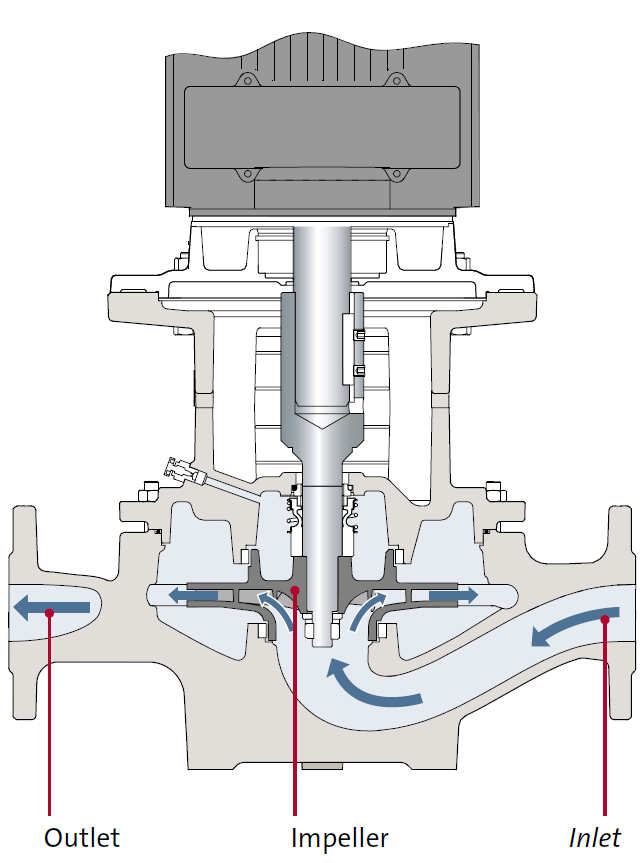
\includegraphics[width=0.4\linewidth]{figures/pump_cross_section.PNG}}}
    \qquad
    \hfill
    \subfloat[Transverse Section]{{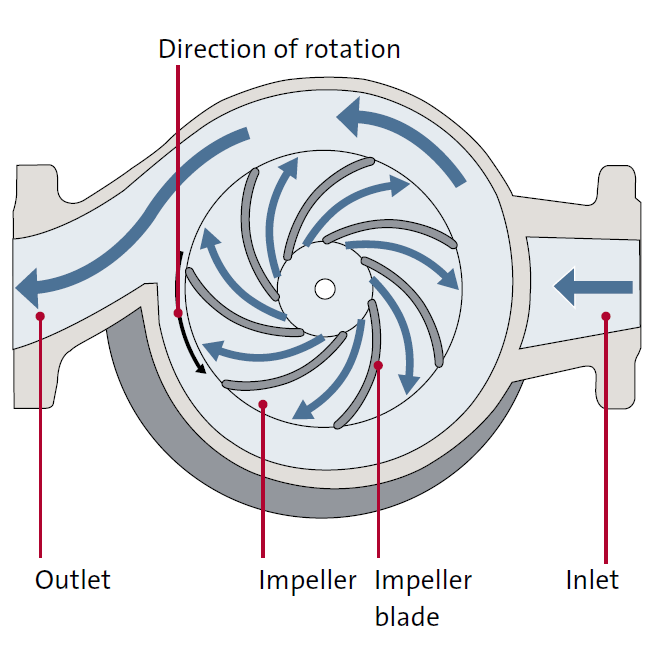
\includegraphics[width=0.4\linewidth]{figures/pump_above_view.PNG}}}
    \caption{Centrifugal Pump}
    \label{fig:pump_sections}
\end{figure}

\subsection{Affinity Laws}
Affinity laws are mathematical relationships that provide a way to estimate the changes in performance of a pump, as a result
of a change in one of the basic pump variables.
In it's simplest form, the term law, means a principle that has been proven true for all cases.
\todo{add affinity laws, formula and statement}
\subsection{Performance Curves}

\section{Pipes}

\section{Valves}

\section{Sensors}